%%%%%%%%%%%%%%%%%%%%%%%%%%%%%%%%%%%%%%%%%
% Jacobs Landscape Poster
% LaTeX Template
% Version 1.1 (14/06/14)
%
% Created by:
% Computational Physics and Biophysics Group, Jacobs University
% https://teamwork.jacobs-university.de:8443/confluence/display/CoPandBiG/LaTeX+Poster
% 
% Further modified by:
% Nathaniel Johnston (nathaniel@njohnston.ca)
%
% This template has been downloaded from:
% http://www.LaTeXTemplates.com
%
% License:
% CC BY-NC-SA 3.0 (http://creativecommons.org/licenses/by-nc-sa/3.0/)
%
%%%%%%%%%%%%%%%%%%%%%%%%%%%%%%%%%%%%%%%%%

%----------------------------------------------------------------------------------------
%	PACKAGES AND OTHER DOCUMENT CONFIGURATIONS
%----------------------------------------------------------------------------------------

\documentclass[final]{beamer}

\usepackage[scale=1.1]{beamerposter} % Use the beamerposter package for laying out the poster
\usetheme{confposter} % Use the confposter theme supplied with this template
\setbeamercolor{block title}{fg=ngreen,bg=white} % Colors of the block titles
\setbeamercolor{block body}{fg=black,bg=white} % Colors of the body of blocks
\setbeamercolor{block alerted title}{fg=white,bg=dblue!70} % Colors of the highlighted block titles
\setbeamercolor{block alerted body}{fg=black,bg=dblue!10} % Colors of the body of highlighted blocks
% Many more colors are available for use in beamerthemeconfposter.sty

%-----------------------------------------------------------
% Define the column widths and overall poster size
% To set effective sepwid, onecolwid and twocolwid values, first choose how many columns you want and how much separation you want between columns
% In this template, the separation width chosen is 0.024 of the paper width and a 4-column layout
% onecolwid should therefore be (1-(# of columns+1)*sepwid)/# of columns e.g. (1-(4+1)*0.024)/4 = 0.22
% Set twocolwid to be (2*onecolwid)+sepwid = 0.464
% Set threecolwid to be (3*onecolwid)+2*sepwid = 0.708

\newlength{\sepwid}
\newlength{\onecolwid}
\newlength{\twocolwid}
\newlength{\threecolwid}
\setlength{\paperwidth}{45in} % A0 width: 46.8in
\setlength{\paperheight}{42in} % A0 height: 33.1in
\setlength{\sepwid}{0.005\paperwidth} % Separation width (white space) between columns
\setlength{\onecolwid}{0.22\paperwidth} % Width of one column
\setlength{\twocolwid}{0.445\paperwidth} % Width of two columns%was 0.464
\setlength{\threecolwid}{0.67\paperwidth} % Width of three columns
\setlength{\topmargin}{-0.5in} % Reduce the top margin size
%-----------------------------------------------------------

\usepackage{graphicx}  % Required for including images
\usepackage{booktabs} % Top and bottom rules for tables
\usepackage{framed, caption}
%----------------------------------------------------------------------------------------
%	TITLE SECTION 
%----------------------------------------------------------------------------------------

\title{A Monte-Carlo based approach for estimating \\remote sensing reflectance uncertainty} % Poster title

\author{Erdem M. Karak\"{o}yl\"{u} \and Bryan Franz} % Author(s)
\institute{NASA Goddard Space Flight Center, Greenbelt, MD, 20771} % Institution(s)

%----------------------------------------------------------------------------------------

\begin{document}

\addtobeamertemplate{block end}{}{\vspace*{2ex}} % White space under blocks
\addtobeamertemplate{block alerted end}{}{\vspace*{2ex}} % White space under highlighted (alert) blocks

%\setlength{\belowcaptionskip}{2ex} % White space under figures
\setlength\belowdisplayshortskip{2ex} % White space under equations

\begin{frame}[t] % The whole poster is enclosed in one beamer frame

\begin{columns}[t] % The whole poster consists of three major columns, the second of which is split into two columns twice - the [t] option aligns each column's content to the top

%\begin{column}{\sepwid}\end{column} % Empty spacer column

\begin{column}{\onecolwid} % The first column

%----------------------------------------------------------------------------------------
%	OBJECTIVES
%----------------------------------------------------------------------------------------

\begin{alertblock}{Objectives}

\begin{itemize}
\item Implement self-contained sensor-dependent (SeaWiFS showcased) noise model.
\item Characterize noise propagation due to atmospheric correction.
\item Characterize impact of noise in near-infrared bands
\item Generate remote sensing reflectance uncertainty product.
\end{itemize}

\end{alertblock}

%----------------------------------------------------------------------------------------
%	INTRODUCTION
%----------------------------------------------------------------------------------------

\begin{block}{Introduction}
\begin{itemize}
\item Satellite borne ocean color remote sensors measure \textbf{top-of-the-atmosphere radiance ($L_T$)}
\item $L_T$ is used to derive \textbf{remote sensing reflectance ($Rrs$)}, from which other  properties of interest are obtained.
\item Typical uncertainty estimation done using potentially problematic comparisons with in-situ data or other remote sensing missions\cite{BW:2006,Tle:2000,Hu:2013}.
\item Consequently a product characterizing $Rrs$ uncertainty has remained illusive.
\end{itemize}
\end{block}

%----------------------------------------------------------------------------------------
%	METHODS - ditch that change to Approach
%----------------------------------------------------------------------------------------

\begin{block}{Approach}
\begin{itemize}
\item All data shown is from the SeaWiFS mission.
\item Signal to noise Ratio (SNR) is modeled (Figure.1) as a function of measured $L_T$
\item Spread in noise distribution is given by $\sigma = \frac{L_T}{SNR}$.
\item A perturbed $L_{T,noise}$ is drawn from $\mathcal{N}(L_T, \sigma)$
\end{itemize}

\begin{framed}
\captionof{figure}{Modeling SNR as a function of $L_T$. Black line is the SNR model. The purple histogram illustrates the relationship of actual data (here, from an open ocean granule) to the model.  }
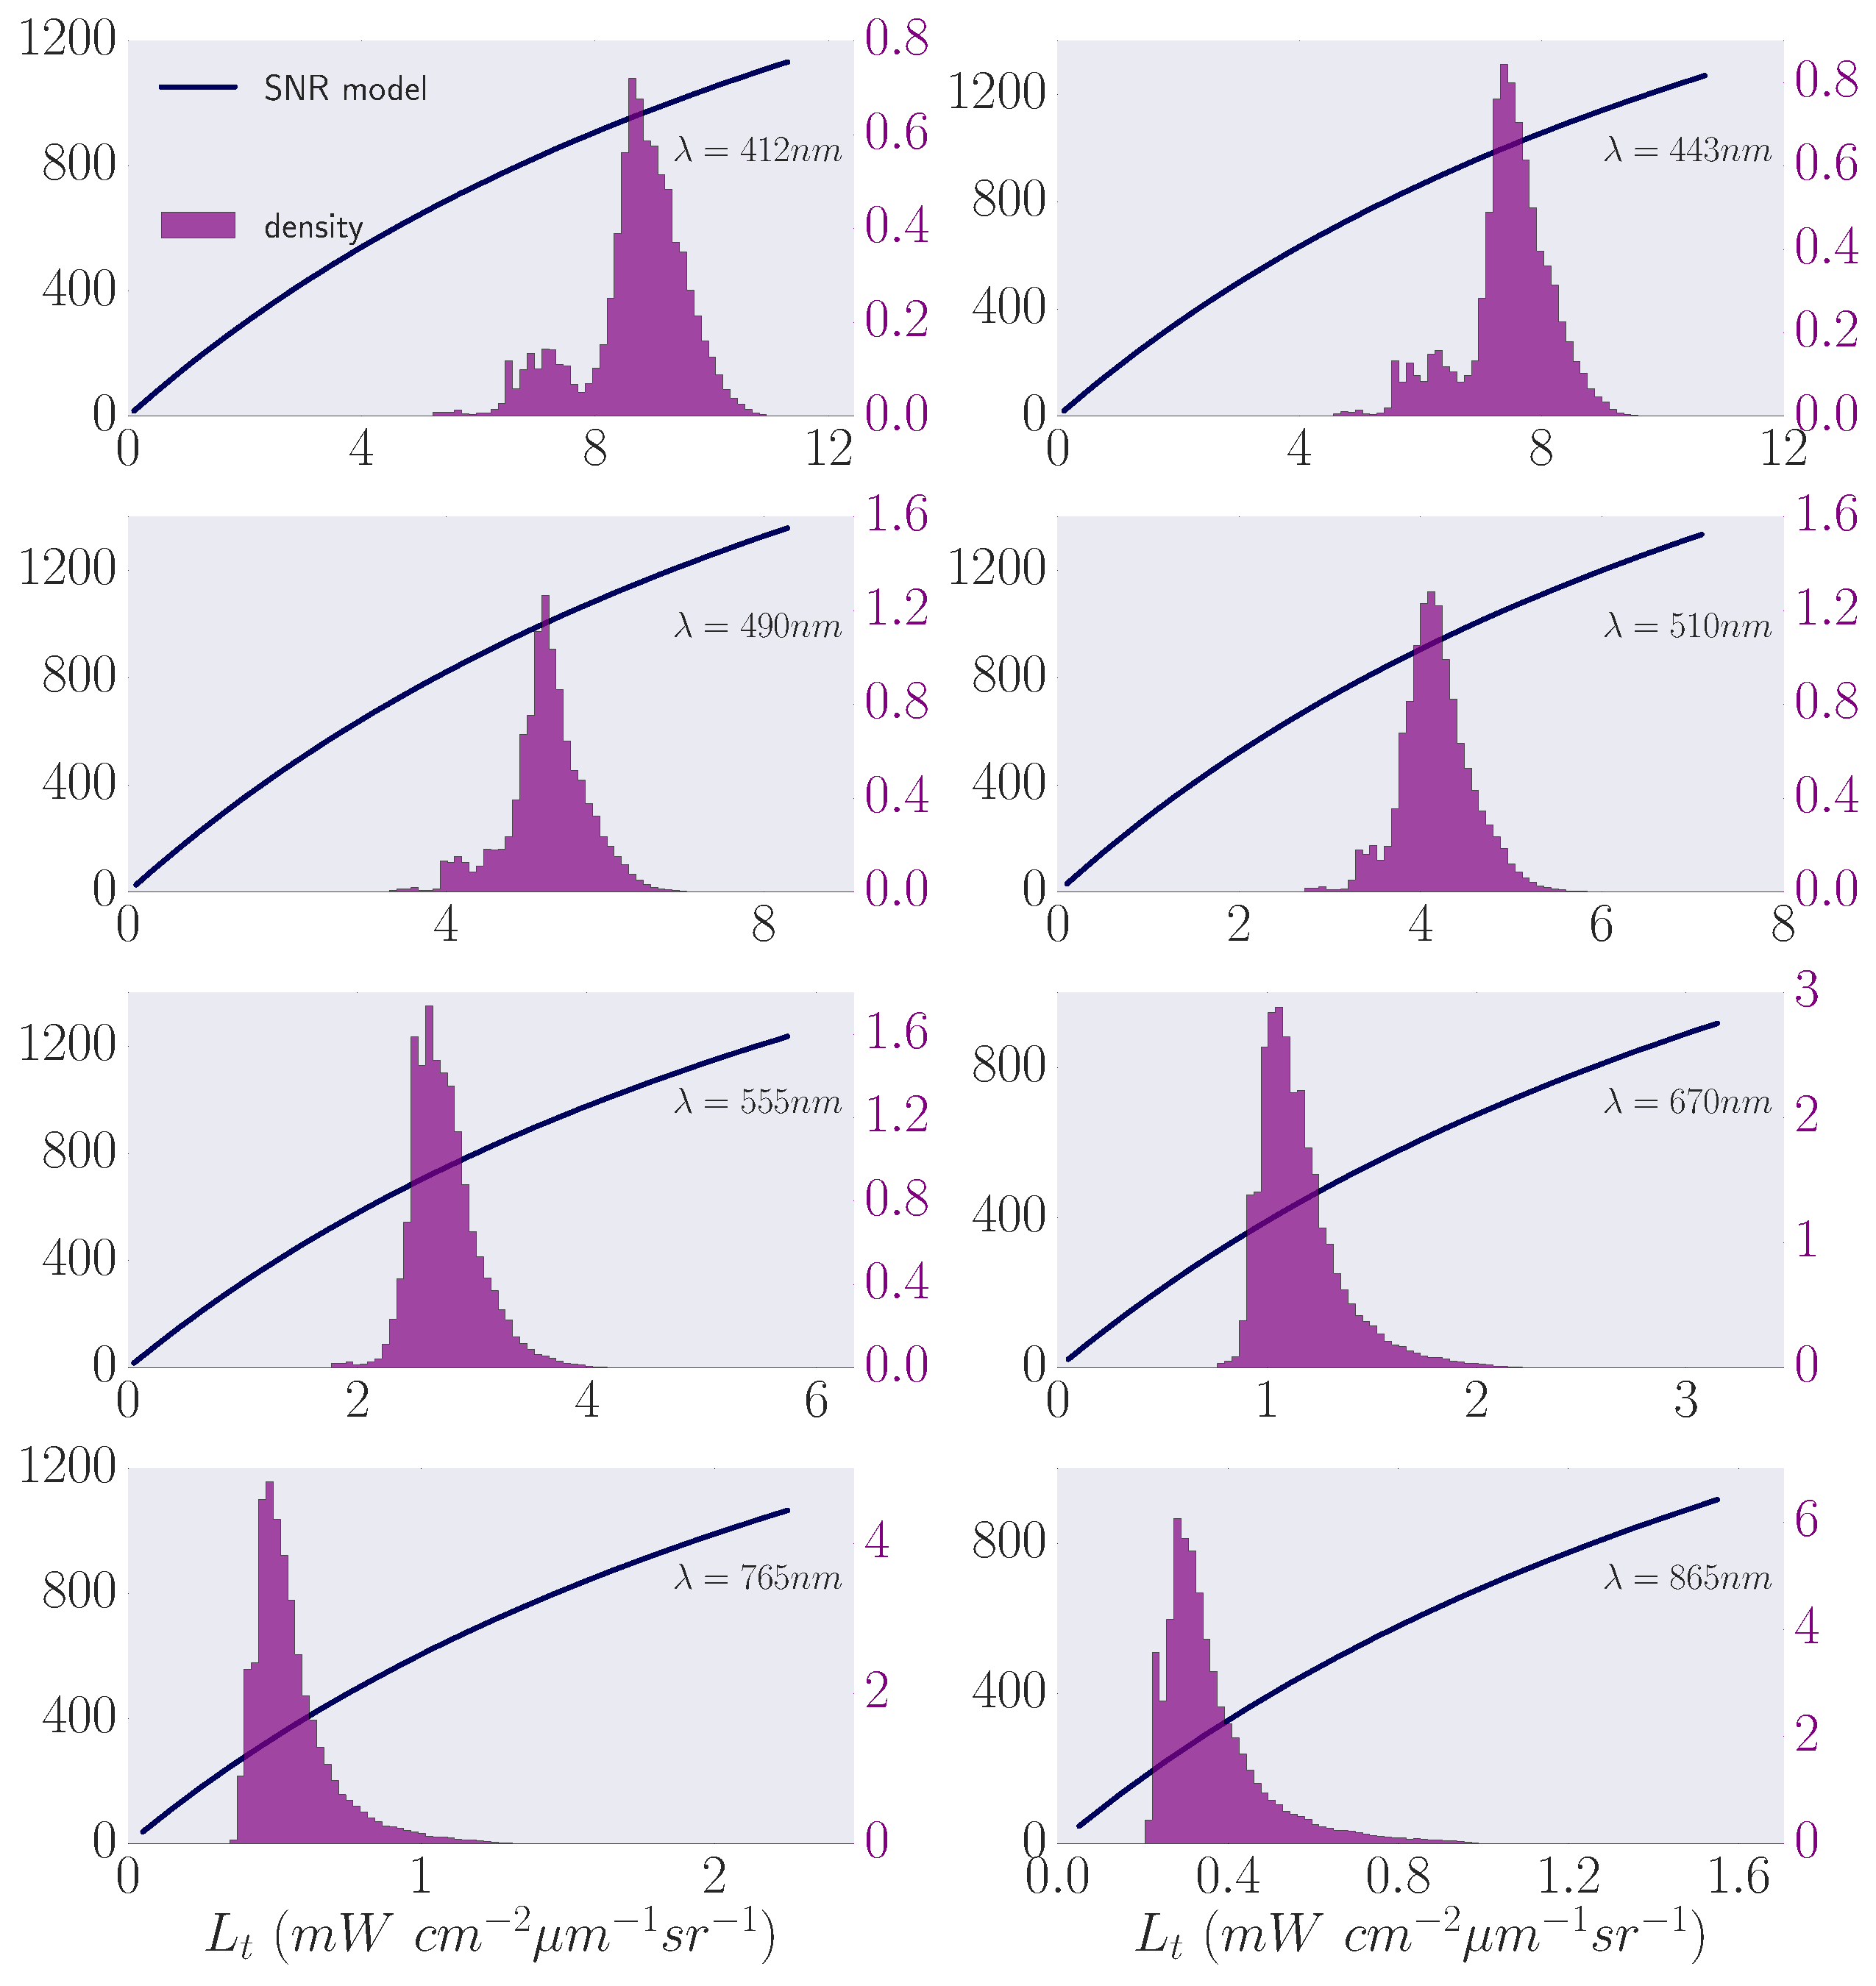
\includegraphics[width=1.0\linewidth]{snrmodelLong.pdf}
\label{fig:snf model}
\end{framed}
\end{block}

\end{column} % End of the first column

%\begin{column}{0.5\sepwid}\end{column} % Empty spacer column

\begin{column}{\twocolwid} % Begin a column which is two columns wide (column 2)
%----------------------------------------------------------------------------------------
%	RESULTS - remove sensitivity analysis figures here, 
%  Do some side by side comparisons of distributions of 
%  Rrs_unc for 
%----------------------------------------------------------------------------------------
\begin{block}{Results}
% ------- NOISE MODEL

% Add sensitivity analysis after this, just one of the plots.
\begin{columns}[t,totalwidth=\twocolwid] % Split up the two columns wide column
% text here?
\begin{column}{\onecolwid}\vspace{-.6in} 
%------------------------------ The first column within column 2 (column 2.1)
%\begin{table}
\begin{framed}
\begin{center}
\vspace{2ex}
\begin{tabular}{|*{7}{c|}}
\toprule
\textbf{Perturbed} & \multicolumn{6}{|c|}{\textbf{\% change in Rrs}}\\
\cline{2-7}
\textbf{Lt} (+0.1\%) & \textbf{412} & \textbf{443} & \textbf{490} & \textbf{510} & \textbf{555} & \textbf{670}\\
\midrule
Lt(412) &  1.14 & -- & -- & -- & -- & --\\  
Lt(443) & 0.22 & 0.97 & 0.21 & 0.22 & 0.22 &  0.53\\
Lt(490) & 0.22 & 0.21 & 0.79 & 0.22 & 0.23 &  0.93\\
Lt(510) & 0.97 & 0.62 & 0.41 &  1.0 & 0.35 & 0.84\\
Lt(555) & 0.23 & 0.22 & 0.23 & 0.24 & 1.6 & 1.2\\
Lt(670) & 0.51 & 0.38 & 0.27 & 0.32 & 0.31 &  5.0\\
Lt(765) & 0.90 & 0.92 & 0.95 &  1.5 &  2.4 &  7.5\\
Lt(865) & 0.66 & 0.65 & 0.65 &  1.0 &  1.5 &  4.3\\
\bottomrule
\end{tabular}
\captionof{table}{Average Rrs response to single-band one-time perturbation. Note that for  $\lambda$>412 there  Predictably, the main diagonal shows larger responses in each row, reflecting the band that was perturbed. However, some of the largest responses can be observed across all bands following perturbations of near-infra red bands ($L_T(765)$ and $L_T(865)$. These are instrumental in the atmospheric correction applied to obtained Rrs}
\end{center}
%end{table}
\end{framed}
\end{column} 
% --------------------------- End of column 2.1
\begin{column}{0.5\sepwid}\end{column} % Empty spacer column
\begin{column}{\onecolwid}\vspace{-.6in} % The second column within column 2 (column 2.2)

\vspace{3ex}
\begin{framed}
\captionof{figure}{ Difference in $Rrs$ response between an MC simulation with visible and near infra-red bands are perturbed and one where only visible bands are perturbed.}
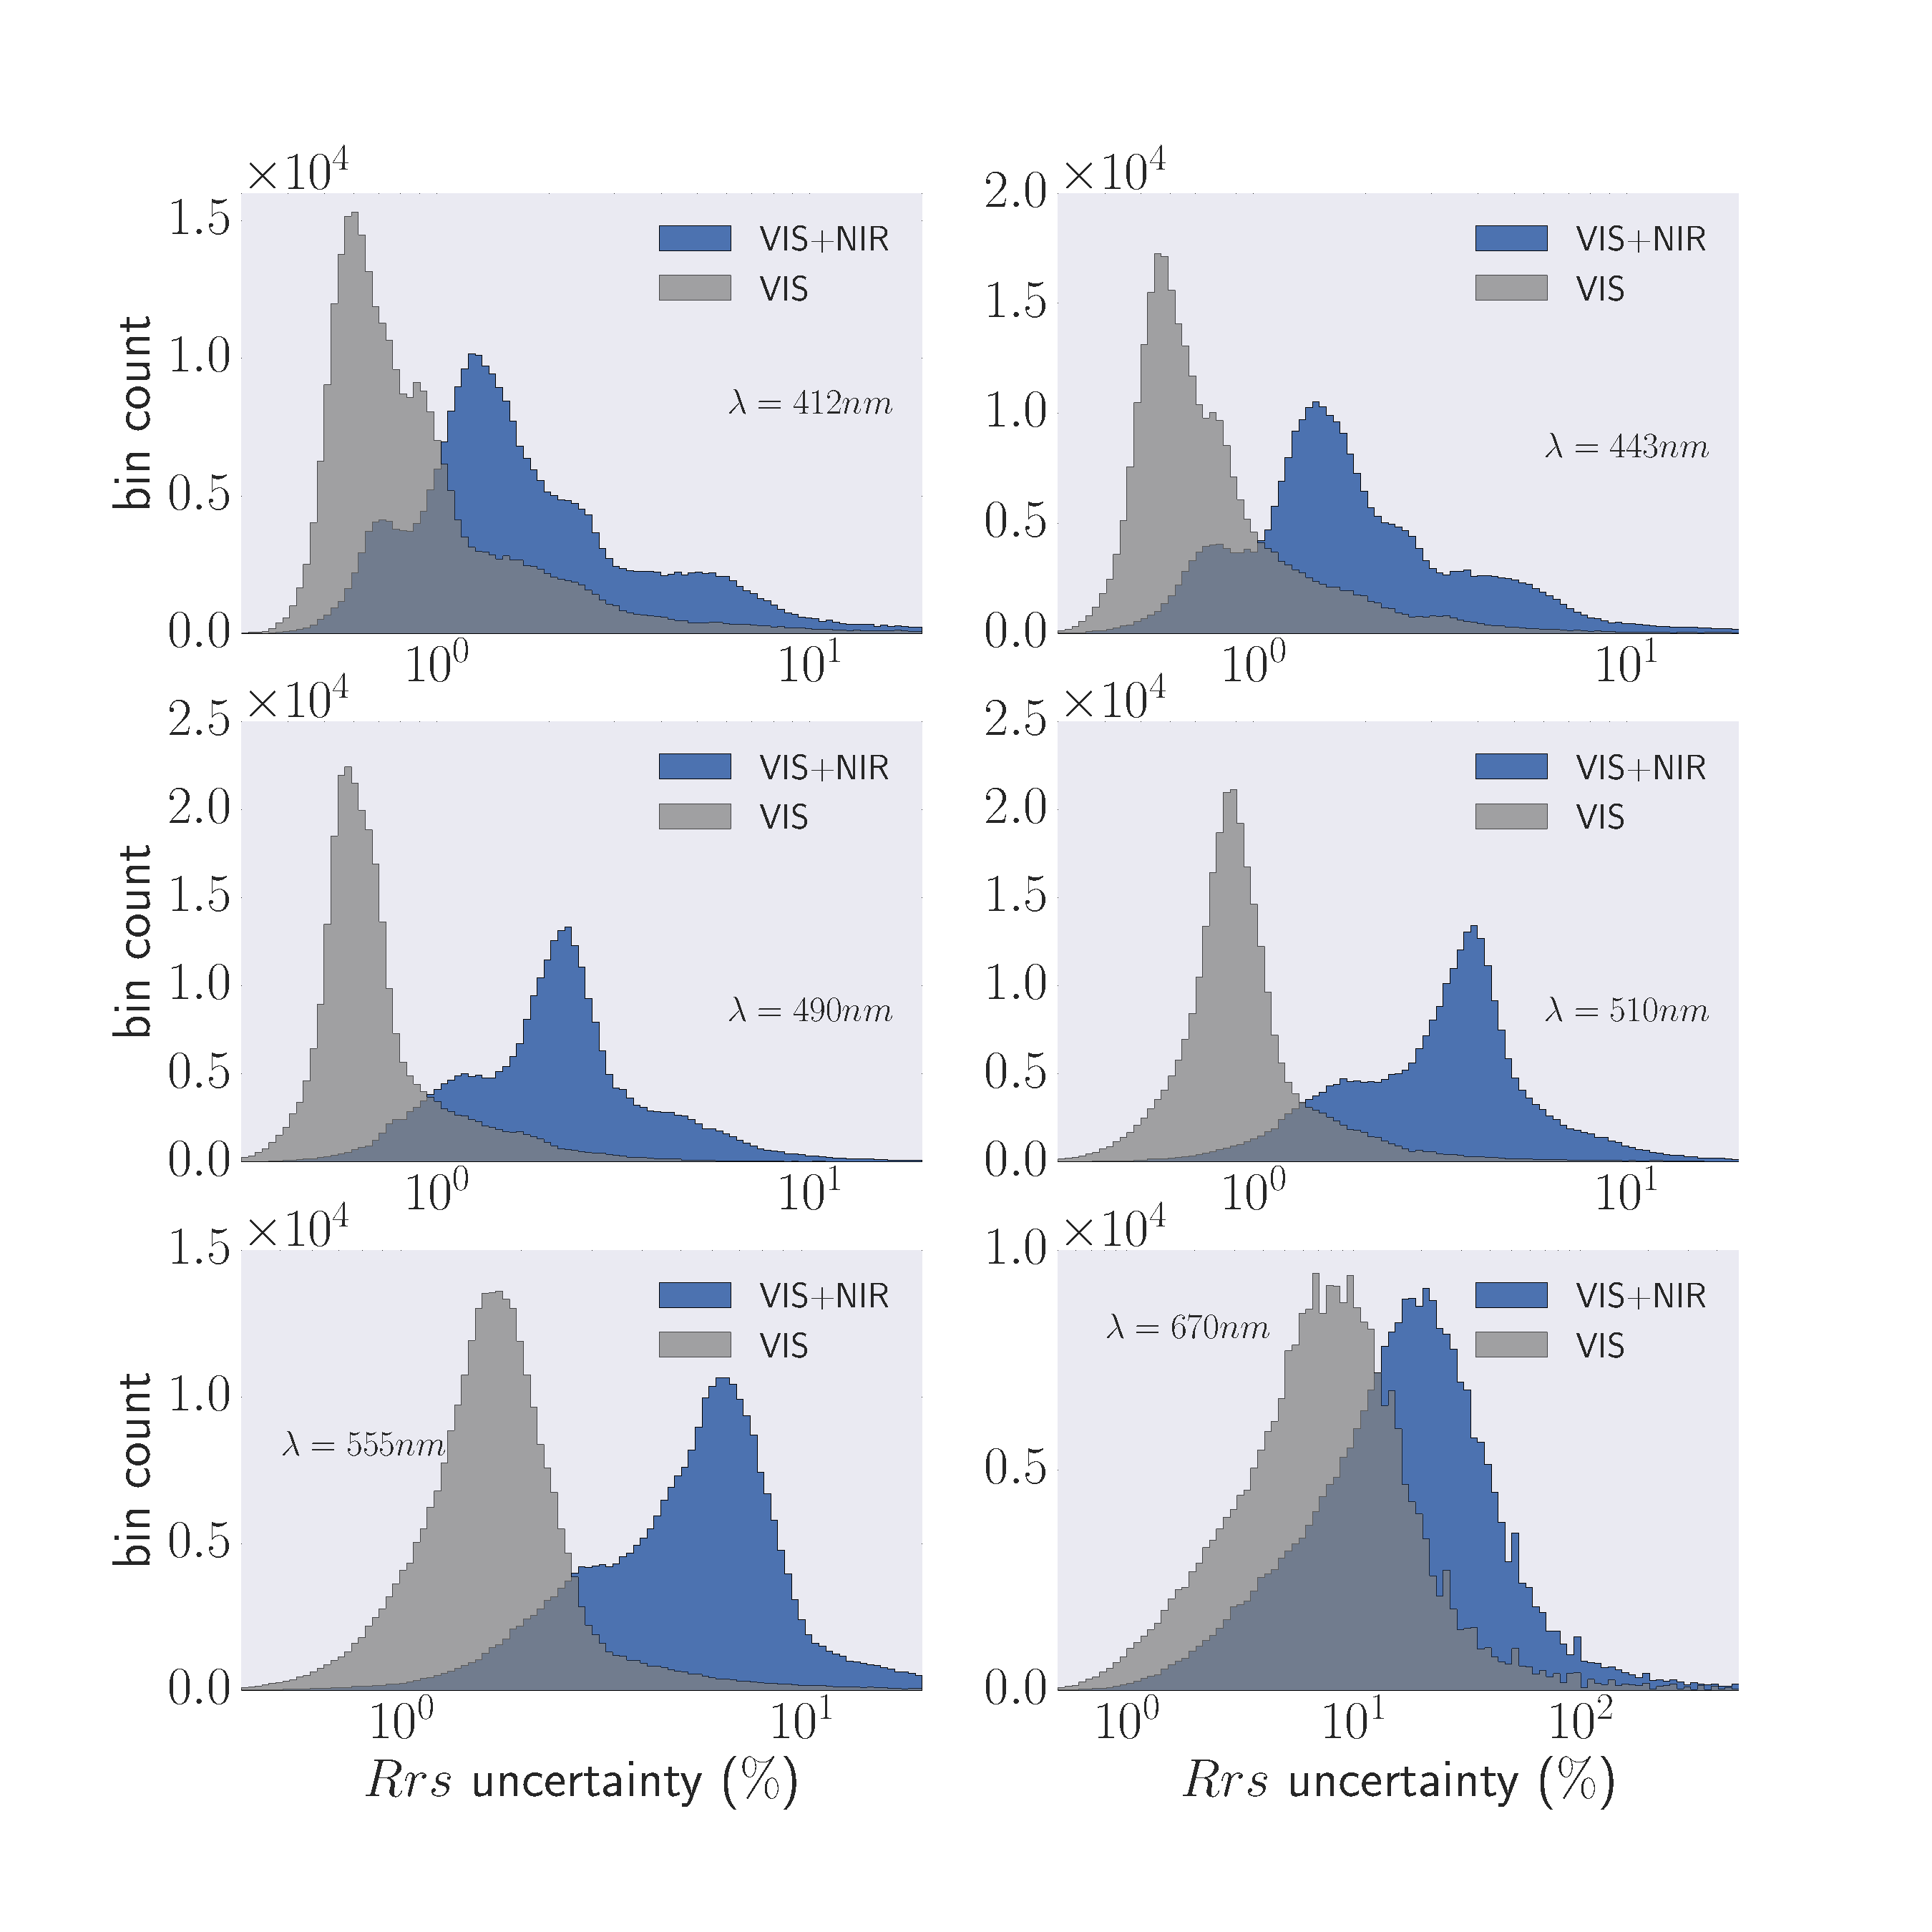
\includegraphics[trim =0 0 0 100,clip,width=1.1\linewidth]{Vis_vs_VISNIR.pdf}
\end{framed}

\end{column} % End of column 2.2

\end{columns} % End of the split of column 2 - any content after this will now take up 2 columns width

\end{block}
%---------- First Global ------------------------
\begin{framed}
\begin{center}
\captionof{figure}{Rrs uncertainty calculated for a global scene -- date--, resulting from a 1000-run MC simulation. Top panel: $Rrs(412 - blue)$ uncertainty. Bottom panel: $Rrs(555)$ uncertainty. Both images are on the same scale (\textit{cf.} color bar). Areas of high radiance in the corresponding band (e.g. open ocean in the case of $Rrs(412)$) are more likely to result in lower uncertainty  and vice versa. }
\includegraphics[width=1.0\linewidth,height=20cm]{rrsPercUnc412.png}
%\end{figure}

%---------- Colorbar ------------------------
%\begin{figure}

\includegraphics[trim =0 10 0 50,clip,width=0.5\linewidth,keepaspectratio]{rrsUNCcolorbar.png}
%\end{figure}

%\begin{figure}

%\caption{Rrs(555) uncertainty (\%)}
\includegraphics[trim =0 0 0 0,clip,width=1.0\linewidth,height=20cm]{rrsPercUnc555.png}
\end{center}
\end{framed}

\begin{columns}[t,totalwidth=\twocolwid] % Split up the two columns wide column again
\begin{column}{\onecolwid} % The first column within column 2 (column 2.1)






%----------------------------------------------------------------------------------------

\end{column} % End of column 2.2

\end{columns} % End of the split of column 2

\end{column} % End of the second column

%\begin{column}{\sepwid}\end{column} % Empty spacer column

\begin{column}{\onecolwid} % The third column

%----------------------------------------------------------------------------------------
%	Summary
%----------------------------------------------------------------------------------------
\begin{block}{Summary}
\begin{itemize}
\item $L_T$ noise amplifies $10x - 70x$ as it propagates to $Rrs$
\item Noise propagation is subject to cross-band contamination.
\item NIR bands (atmospheric correction) contribute significantly  noise amplification 
\item MC simulation converges successfully to yield Rrs uncertainty 
\item For real $L_T$ data
\item Higher uncertainty found in complex coastal waters
\end{itemize}
\end{block}
%----------------------------------------------------------------------------------------
%	What's next?
%----------------------------------------------------------------------------------------

\begin{block}{Next...}
\begin{itemize}
\item Extend MC simulations to other sensors.
\item MC simulations computationally costly;
	\begin{itemize}
	\item Finding an alternative to build on this work, a priority
	\item Develop machine learning (ML) approach (e.g. neural network);
	\item Identify uncertainty drivers in MC as potential inputs to ML;
 	\item Use ML to shorten uncertainty product generation to one run. 
	\end{itemize}
\end{itemize}

\end{block}


%----------------------------------------------------------------------------------------
%	REFERENCES
%----------------------------------------------------------------------------------------

\begin{block}{References}
\nocite{} % Insert publications even if they are not cited in the poster
\small{\bibliographystyle{IEEEtran}
\bibliography{poster}\vspace{0.75in}}

\end{block}

%----------------------------------------------------------------------------------------
%	ACKNOWLEDGEMENTS
%----------------------------------------------------------------------------------------

\setbeamercolor{block title}{fg=red,bg=white} % Change the block title color

\begin{block}{Acknowledgements}

\small{\rmfamily{We thank \textit{Don Shea} and \textit{Sean Bailey} for assistance with l2gen integration of the MC code, and to \textit{Tommy Owens} for running large scale MC simulations on the OBPG production system.}} \\

\end{block}

%----------------------------------------------------------------------------------------
%	CONTACT INFORMATION
%----------------------------------------------------------------------------------------

\setbeamercolor{block alerted title}{fg=black,bg=norange} % Change the alert block title colors
\setbeamercolor{block alerted body}{fg=black,bg=white} % Change the alert block body colors

\begin{alertblock}{Contact Information}

\begin{itemize}
\item Web: \href{oceancolor.gsfc.nasa.gov}{oceancolor.gsfc.nasa.gov}
\item Email: \href{mailto:erdem.m.karakoylu@nasa.gov}{erdem.m.karakoylu@nasa.gov}
\item Phone: +1 (301) 286 0501
\end{itemize}

\end{alertblock}

\begin{center}
\begin{tabular}{ccc}

\includegraphics[width=0.4\linewidth]{NASA_logo.png} & \hfill 
\end{tabular}
\end{center}

%----------------------------------------------------------------------------------------

\end{column} % End of the third column
\begin{column}{\sepwid}\end{column} % Empty spacer column
\end{columns} % End of all the columns in the poster

\end{frame} % End of the enclosing frame

\end{document}
